\section{Метод конечных разностей во временной области}

Методы конечных разностей для зависимых от времени дифференциальных уравнений в частных производных давно используются в решении задач вычислительной гидродинамики. Метод конечных разностей во временной области (FDTD) является логичным обобщением подобных алгоритмов на поле задач электродинамики. Он был разработан \cite{Yee1966} Кейном Йи (англ. Kane S. Yee) в 1966 году и его ключевым результатом является определение полей $E, H$ на дискретной по времени сетке.

Алгоритм Йи основывается на дискретизации уравнений Максвелла:

\begin{equation}
  \frac{\partial \vec{B}}{\partial t} = - \nabla \times \vec{E}
  \label{eq:maxwell_B}
\end{equation}

\begin{equation}
  \frac{\partial \vec{D}}{\partial t} + \vec{J}(\vec{r}, t) = \nabla \times \vec{H}
  \label{eq:maxwell_D}
\end{equation}

\begin{equation}
  \vec{B} = \mu(\vec{r}, t)\vec{H}
\end{equation}

\begin{equation}
  \vec{D} = \varepsilon(\vec{r}, t)\vec{E}
\end{equation}

Следует обратить внимание, что $\vec{J}, \mu$ и $\varepsilon$ зависят от радиус-вектора и от времени.

\begin{figure}[h]
	\centering
	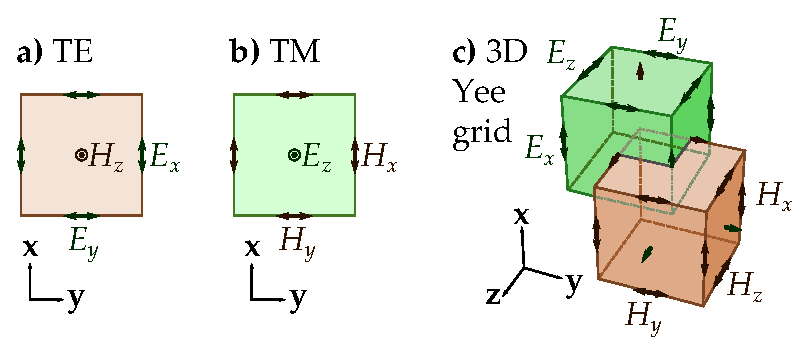
\includegraphics{img/FDTD_Yee_grid_2d_3d}
	\caption{Пространственная сетка в методе Йи}
	\label{fig:fdtd}
\end{figure}

Для дискретизации уравнений Максвелла Йи предложил сетку, изображённую на рисунке \ref{fig:fdtd}, причём сетки для полей $E$ и $H$ смещены по отношению друг к другу на полшага не только по пространственным координатам, но и по времени.

\begin{equation}
  \brround{i, j, k} = \brround{i\Delta x, j\Delta y, k\Delta z}
\end{equation}

Тогда функция $F(x, y, z, t)$ превратится в

\begin{equation}
  F\brround{i\Delta x, j\Delta y, k\Delta z, n\Delta t} = F^{(n)}\brround{i,j,k} 
\end{equation}

Из чего, к примеру, следует следующий вид уравнения \ref{eq:maxwell_B} для $B_x$

\begin{multline}
	\frac{B_x^{n+1/2}(i,j+1/2,k+1/2)-B_x^{n-1/2}(i,j+1/2,k+1/2)}{\Delta t} = \\
	= \frac{E_y^n(i, j+1/2,k+1) - E_y^n(i, j+1/2,k)}{\Delta z} - \frac{E_z^n(i, j+1,k+1/2) - E_z^n(i,j,k+1/2)}{\Delta y},
\end{multline}

а уравнение \ref{eq:maxwell_D} для $D_x$ запишется как

\begin{multline}
	\frac{D_x^n(i+1/2,j,k) - D_x^{n-1}(i+1/2,j,k)}{\Delta t} + J_x^{n-1/2}(i+1/2,j,k)= \\
	= \frac{H_z^{n-1/2}(i+1/2,j+1/2,k) - H_z^{n-1/2}(i+1/2,j-1/2,k)}{\Delta y} - \\
	- \frac{H_y^{n-1/2}(i+1/2,j,k+1/2) - H_y^{n-1/2}(i+1/2,j,k-1/2)}{\Delta z}
\end{multline}

Важной частью получения численного решения является задание граничных условий. Существуют два наиболее часто используемых типов условий -- поглощающие (PML) или периодические. Условия первого типа используются при моделировании затухания волны на бесконечности, а второй тип условий используется при расчёте параметров периодических структур.

Существует несколько независимых реализаций метода конечных разностей во временной области. Одним из самых мощных и удобных подобных инструментов является программный пакет Lumerical FDTD Solutions, который и использовался в данной работе.

Примерный алгоритм использования Lumerical FDTD Solutions может выглядеть следующим образом:

\begin{enumerate}[label=\arabic*)]
	\item Задание исследуемых структур. Выбор форм и материалов.
	\item Выбор подходящих источников электромагнитного излучения (включая их профиль, длительность импульса и спектр).
	\item Выбор граничных условий.
	\item Выбор области расчёта.
	\item Задание ``мониторов'' - областей, в которых будут зафиксированы рассчитанные параметры поля.
	\item Расчёт.
\end{enumerate}

Также в данной работе для итерации по области параметров использовалась встроенная функция интерпретации скриптов, позволяющая осуществлять расчёты в полуавтоматическом режиме.